\documentclass[11pt,a4paper]{article}
\usepackage{fontspec}
\setmainfont{NotoSerifCJKkr-Regular.otf}[Path=fonts/,BoldFont=NotoSerifCJKkr-Bold.otf,ItalicFont=NotoSerifCJKkr-Regular.otf]
\setsansfont{NotoSerifCJKkr-Regular.otf}[Path=fonts/,BoldFont=NotoSerifCJKkr-Bold.otf]
\setmonofont{DejaVu Sans Mono}[Scale=0.79]
\XeTeXlinebreaklocale "ko"
\XeTeXlinebreakskip=0pt plus 1pt
\usepackage[margin=23mm,top=24mm,bottom=24mm,headheight=15pt]{geometry}
\usepackage{amsmath,amssymb,amsthm,mathtools}
\usepackage{booktabs,tabularx,longtable,array,graphicx,float}
\usepackage[dvipsnames]{xcolor}
\usepackage{enumitem,caption,fancyhdr,titlesec}
\usepackage{hyperref}
\hypersetup{unicode=true,colorlinks=true,linkcolor=MidnightBlue,urlcolor=MidnightBlue,citecolor=MidnightBlue,pdftitle={WU088 HH PHYS14: 공동 carry와 두 번째 half},pdfauthor={WU088 HH 연구}}
\urlstyle{same}
\setlength{\emergencystretch}{3em}
\setlength{\parskip}{0.35em}
\setlength{\parindent}{1em}
\widowpenalty=10000
\clubpenalty=10000
\linespread{1.12}
\setlist{itemsep=0.15em,topsep=0.4em,leftmargin=1.6em}
\captionsetup{font=small,labelfont=bf}
\renewcommand{\figurename}{그림}
\renewcommand{\tablename}{표}
\renewcommand{\refname}{원문 근거와 재현 자료}
\titleformat{\section}{\large\sffamily\bfseries\color{MidnightBlue}}{\thesection}{0.7em}{}
\titleformat{\subsection}{\sffamily\bfseries}{\thesubsection}{0.7em}{}
\pagestyle{fancy}\fancyhf{}
\fancyhead[L]{\small\sffamily WU088\_HH / PHYS14}
\fancyhead[R]{\small\sffamily 2026-10-12}
\fancyfoot[C]{\thepage}
\newcommand{\HH}{\mathrm{HH}}
\newcommand{\fh}{\widehat f}
\newcommand{\R}{\mathsf R}
\newcommand{\dd}{\mathrm d}
\newcommand{\ee}{\mathrm e}
\newcommand{\vu}{\nu_H}
\newcommand{\Np}{N^{\mathrm{in}}}
\newcommand{\parth}{\partial_\lambda}
\newtheorem{proposition}{명제}
\begin{document}
\begin{center}
{\color{MidnightBlue}\sffamily\large WU088\_HH \quad PHYS14}\par
\vspace{5mm}
{\LARGE\bfseries 공동 carry의 두 번째 half 전달과\\[0.25em]광자 기억의 온도 응답}\par
\vspace{4mm}
{\large 등방 39개 상태 축약, 유일 근, 혼합 응답 및 원 격자의 수송 분할}\par
\vspace{2mm}
2026년 10월 12일
\end{center}
\vspace{2mm}
\noindent\rule{\textwidth}{0.6pt}

\section*{초록}
PHYS11의 공동 기체·광자 carry와 PHYS13의 첫 half 근 포함을 실제 두 번째 half 암시적 단계로 전달했다. 같은 COMMON에서 출발하여 두 half에 공통 미래 제어변수 $(\lambda,b)\in[0,1]^2$를 적용했다. 원 등방 기하학과 33개 에너지 node에서 ray 합을 취하면 기체 4개, photon group 33개, 총 guard 2개로 이루어진 39개 실수 상태가 정확히 닫힌다. 이 축약을 이용하여 새 단계의 incoming, 흡수 denominator, 잔차와 도함수를 구성했다.

원 source domain에서 strict self-map과 $\kappa<5.393\times10^{-4}$를 확인했다. 따라서 상속한 첫 단계와 같은 $C^2$ 계열의 다음 유일 근을 포함한다. 이어진 두-half endpoint의 유한 HH 온도 응답은 $[-18.93685,-9.75153]\,\mu\mathrm K$이고 전자 수 응답은 $[1.34316,2.59529]\times10^{-10}\,\mathrm{electrons/H}$다. 추가 광자 birth의 온도 응답도 음수이며, HH--birth 혼합 온도 응답은 $[1.96632,3.44806]\,\mathrm{pK}$로 양수다.

HH 첫 미분을 전달 기체, 현재 직접 HH, 전달 광자 기억으로 분해했다. 광자 기억은 현재 열에너지를 늘리면서 온도를 $[0.49244,1.64910]\,\mathrm{pK}$만큼 추가로 낮추는 방향이다. 이는 실제 33개 group의 signed carry를 모두 포함한 결과다.

별도로 원 비균일 격자의 $\R(\rho)^2-\R(\rho^2)$를 정확히 유도했다. 광자수·에너지 moment가 0이어도 spectral shape가 달라진다. 현재 최소 node 간격 부근의 최대 column $\ell^1$ 차이는 약 $0.754776$이고, 실제 COMMON에 가중한 HI 활성 node의 광자수 차이는 약 $-8.681\times10^{-9}\,\mathrm{photons/H}$다. 이 수송 연산자 진단과 완전한 기체 endpoint 차이는 구별한다.

수치 범위는 원 고정 계수의 실수 source와 첫 단계 포함을 상속한 등방 geometric subfamily에 해당한다. 이번에는 새 암시적 단계 한 개를 검증된 구간 계산으로 실행했으며, native 상태 권한이나 전역 EoR 적용 판정은 별도 경로에 남는다.\cite{result,theory,review}

\section{연구 질문과 상속한 이력}
PHYS13은 같은 COMMON에서 따로 시작하는 Full과 first\_half의 온도·전자 응답을 정리했다. PHYS14의 질문은 첫 half가 남긴 기체와 광자의 값 및 $U,V,W$를 함께 전달했을 때, 다음 half에서도 HH 냉각과 혼합 응답의 부호가 유지되는가이다. 두 개의 독립 첫 단계 결과를 더하는 방법은 이 질문의 이력을 구성하지 않는다. 이번에는 PHYS11의 실제 first\_half outgoing joint carry를 다음 incoming으로 사용했다.\cite{phys11,phys13}

\begin{equation}
 t_0=1.6\times10^{11}\,\mathrm s,\quad h=6.25\times10^8\,\mathrm s,\quad
 t_1=t_0+h,\quad t_2=t_0+2h=1.6125\times10^{11}\,\mathrm s.
\end{equation}
과거 HH ON 이력과 COMMON의 primal compensation은 원 입력으로 유지한다. 미래 $\lambda$는 두 half의 HH 항에, $b$는 두 half의 광자 birth에 공통으로 작용한다. 모든 미분과 유한 차이는 같은 계수 묶음과 같은 COMMON을 고정한다.

기체 좌표, 단위와 도함수는
\begin{equation}
g=(x_{\mathrm{HII}},y_{\mathrm{HeII}},y_{\mathrm{HeIII}},w),\qquad
U=\partial_\lambda g,\quad V=\partial_b g,\quad W=\partial_\lambda\partial_b g
\end{equation}
로 둔다. $w$는 $\mathrm{eV/H}$, $N_j$는 $\mathrm{photons/H}$다. 온도·전자 정의에는 원 FT03 source의 저장 밀도비를 사용한다.
\begin{align}
 f&=\operatorname{exact}(f_{\mathrm{He,stage}}),&
 \fh&=\frac{\operatorname{exact}(n_{\mathrm{He,stored}})}{\operatorname{exact}(n_H)},\\
 e&=x+\fh(y_1+2y_2),&\Pi&=1+\fh+e,\\
 T&=C_T\frac{w}{\Pi},&C_T&=\frac{2\operatorname{exact}(\epsilon_{\mathrm{eV}})}{3\operatorname{exact}(k_B)}.
\end{align}
stage $f$와 source $\fh$를 서로 바꾸지 않는다. 기하학의 세 $H_i$는 같은 captured binary64 값 $10^{-14}\,\mathrm{s}^{-1}$다. 수식의 계산 상수는 명시한 captured leaf의 정확한 실수값을 뜻한다.\cite{ncp07,phys13}

\section{등방 배경의 정확한 39개 상태 축약}
원 ray 기하학의 실수 함수는
\begin{equation}
 G_r(t)=\left[\sum_{i=1}^3 q_{ri}^2\ee^{-2H_i t}\right]^{1/2}
 =\ee^{-Ht}\|q_r\|,\qquad \rho=G_r(t+h)/G_r(t)=\ee^{-Hh}
\end{equation}
다. captured $q_r$가 정확한 단위벡터라는 추가 가정은 필요 없다. 모든 ray에 같은 $\rho$가 적용되고, source weight는
\begin{equation}
 \omega_r=\frac{\|q_r\|^{-3}}{\sum_s\|q_s\|^{-3}},\qquad \sum_r\omega_r=1
\end{equation}
로 정상화된다. 독립 검토에서 이 공통 $\rho$와 실제 정상화 weight를 원 ray별 구간 전부에 포함했다. 원본에서는 ray ratio 끝점이 서로 다르므로, 이번 대상은 그 포함 안의 기하학적 관계를 만족하는 subfamily로 명시한다.\cite{geometry}

원 piecewise-linear hat remap을 $\R_{ij}(\rho)=H_i(\rho E_j)$라 쓰면
\begin{equation}
 \Np_2=\R(\rho)N_1^+ + bM e_{24},\qquad
 M=\operatorname{exact}(\operatorname{fl}(h\,\mathrm{SOURCE}))
\end{equation}
가 정확하다. $M$은 원 captured 곱을 그대로 쓰며 새 부동소수점 곱으로 교체하지 않는다. 아래 guard로 나간 광자는 총 number와 energy에 더하고, 기존 guard energy에는 $\rho$를 곱한다. 흡수 denominator도 ray에 독립이므로 $\sum_r n_{r,j}^{\mathrm{in}}/D_j=N_j^{\mathrm{in}}/D_j$다.

\begin{proposition}[등방 aggregate closure]
원 full ray stage의 source-aligned 실수 사상을 $\Phi$, $(g,N,G_N,G_U)$ 합을 취하는 선형 사상을 $\mathsf C$라 하자. 동일한 유일 gas root를 쓰는 aggregate stage $\bar\Phi$에 대해 $\mathsf C\Phi=\bar\Phi\mathsf C$다. 따라서 임의의 연속된 해당 등방 stage에 같은 교환 관계가 성립하고, 값·$U$·$V$·$W$에도 그대로 적용된다.
\end{proposition}
증명은 선형 transport의 유한합 교환, 공통 denominator의 합 교환, 동일 gas residual의 유일성으로 얻는다. 이로써 기체 4개+group 33개+총 guard 2개, 총 39개 상태와 156개 carry slots가 닫힌다. 원 4,484개 상태에서의 대수적 축약이며 실행 속도비의 측정치는 아니다. 원 scalar native의 별도 선행 곱 capture graph는 PHYS11 provenance에 보존한다.\cite{theory,phys11}

\section{새 source와 두 번째 half의 유일 근}
\subsection{기존 source의 재사용 조건}
$t_2$는 기존 Full의 종료 시각이다. 원 source의 density, stored helium, $H_{\rm mean}$ 및 원자 leaf가 이 endpoint에서 같으므로, Full의 nonphoto $F^{\mathrm{np}}$와 HH rate $q$의 값·gas gradient·gas Hessian을 재사용할 수 있다. 이 두 함수에는 $h$, 이전 gas, incoming photon의 직접 의존성이 없다. 새 $h$와 실제 전달 incoming은 다음 식에 넣는다.\cite{source,theory}
\begin{equation}\label{eq:source}
 F_2(g)=F^{\mathrm{np}}(g)+\lambda q(g)\vu
 +\sum_{j=0}^{32}p_j(x)\Np_{2,j}\nu_j-2H_{\rm mean}w e_w,
\end{equation}
\begin{align}
 \vu&=(1,0,0,-\chi_H),&\nu_j&=(1,0,0,\epsilon_j),\\
 a_j&=c n_H\sigma_{j,\mathrm{HI}},&D_j&=1+h a_j(1-x),\\
 p_j&=\frac{a_j(1-x)}{D_j},&p'_j&=-\frac{a_j}{D_j^2},\qquad p''_j=-\frac{2ha_j^2}{D_j^3}.
\end{align}
여기서 $\epsilon_j$는 원 source에 저장된 HI photoelectron 열 초과분 leaf의 정확한 실수값이며 단위는 eV다. 저장된 energy와 $\chi_H$를 새로 빼서 이 leaf를 교체하지 않는다. 실제 sigma bits에서 HI 활성 node는 16--32이고 HeI·HeII photo sigma는 전체 33개에서 0이다. nonphoto의 helium coupling은 식~\eqref{eq:source}에 남는다. Photo gas Jacobian은 $x$ 한 열만 비영인 rank-one 구조다.\cite{result,theory}

원 $X$와 새 근 포함은 표~\ref{tab:root}와 같다. 먼저
\begin{equation}
Y_1+h[F_2](X)\subset\operatorname{int}X,\qquad
\|S^{-1}h[F_{2,g}](X)S\|_\infty\le\kappa<1,\quad
S=\operatorname{diag}(1,1,1,13.5)
\end{equation}
를 확인했다. 원 구간을 포함하는 $X$는 표의 간단한 십진 표기보다 binary64 한두 ulp 넓다. 정확한 끝점은 결과 JSON에 보존한다.
\begin{table}[H]\centering\footnotesize
\caption{기체 domain과 PHYS14 두 번째 half의 근 포함. 새 근은 원 $X$ 내부다.}
\label{tab:root}
\setlength{\tabcolsep}{4pt}
\begin{tabular}{@{}lll@{}}\toprule
좌표 & 원 $X$의 간단 표기 & 새 $g_2$ 포함\\\midrule
$x$ & $[0.90,0.93]$ & $[0.9132202086, 0.9168624395]$\\
$y_1$ & $[0.29,0.31]$ & $[0.2999648443, 0.3000354168]$\\
$y_2$ & $[0.59,0.61]$ & $[0.5999927007, 0.6000072419]$\\
$w$ & $[13,14]$ & $[13.4343397863, 13.5652408859]$\\
\bottomrule\end{tabular}
\end{table}


원 domain 수축 상한은 $0.0005392100481791$이다. source centre의 정확한 captured 좌표 $(0.915,0.3,0.6,13.5)$와 whole-$X$ 도함수를 이용한 Taylor 포함을 교차하고 네 번의 image 교차를 수행한 뒤, 수축 상한은 $0.0005045844357588$로 포함된다. 각 Taylor 선분은 convex $X$에 들어간다. 모든 $D_j>0$, strict self-map 및 uniform inverse에 의해 새 근은 상속한 첫 단계와 같은 $C^2$ 계열을 이룬다.\cite{result,review}

\section{전달된 일차·혼합 미분과 유한 차이}
첫 단계 광자 carry를 수송하면
\begin{equation}
U^{\mathrm{in}}_{N,2}=\R U^+_{N,1},\quad
V^{\mathrm{in}}_{N,2}=\R V^+_{N,1}+M e_{24},\quad
W^{\mathrm{in}}_{N,2}=\R W^+_{N,1}
\end{equation}
이다. incoming의 이전 gas 의존성은 이 carry에 포함되어 있으며, 현재 단계의 gas unknown에 대한 직접 gradient는 0이다. $A=I-hF_{2,g}$라 두면 PHYS11의 공동 chain rule은
\begin{align}
AU_2&=U_1+hF_{2,\lambda},\\
AV_2&=V_1+hF_{2,b},\\
AW_2&=W_1+h\{F_{2,gg}[U_2,V_2]+F_{2,g\lambda}V_2
 +F_{2,gb}U_2+F_{2,\lambda b}\}
\end{align}
로 적용된다. $F_{2,\lambda}$에는 직접 $q\vu$와 $\sum_jp_j\nu_jU^{\mathrm{in}}_{N,j}$가 모두 들어가고, $F_{2,\lambda b}$에는 전달 광자의 mixed carry가 들어간다. 새 $W_2$의 두 교차항에 같은 새 $U_2,V_2$를 사용했다.\cite{phys11,result}

$L=hF_g$에 대해 $\sum_{k=0}^8L^k r$와 다음 tail을 사용하여 세 선형 문제를 포함했다.
\begin{equation}
 |\mathrm{tail}_i|\le S_{ii}\frac{\kappa^9}{1-\kappa}\|S^{-1}r\|_\infty.
\end{equation}
thermal 성분의 tail 상한은 $U,V,W$ 순서로 $7.491\times10^{-39}$, $2.837\times10^{-37}$, $1.786\times10^{-45}$다. 결과 폭의 주원인은 이 tail이 아니라 상속 source/carry 포함이다. 이는 실제 중심값의 통계적 오차나 confidence interval이 아니다.

새 outgoing photon은 $N^+=\Np/D$로 구성했다. 특히
\begin{align}
W_N^+={}&\frac{W_N^{\mathrm{in}}}{D}
 +\frac{ha}{D^2}\left(U_N^{\mathrm{in}}V_x+V_N^{\mathrm{in}}U_x+\Np W_x\right)
 +\frac{2(ha)^2\Np U_xV_x}{D^3}
\end{align}
를 사용한다. 흡수량의 linked 식도 함께 평가했고 33개 group의 네 carry 성분에서 $N^{\mathrm{in}}-N^+-N^{\mathrm{abs}}$ 포함이 0을 포함한다. 이 좌표별 검사는 동일한 물리 case의 산술 assertion이다.\cite{result}

\section{두-half endpoint의 온도·전자 응답}
$U_e=U_x+\fh(U_{y_1}+2U_{y_2})$와 $V_e,W_e$를 정의하면
\begin{align}
U_T&=C_T\left(\frac{U_w}{\Pi}-\frac{wU_e}{\Pi^2}\right),\\
W_T&=C_T\left(\frac{W_w}{\Pi}-\frac{U_wV_e+V_wU_e+wW_e}{\Pi^2}
+\frac{2wU_eV_e}{\Pi^3}\right)
\end{align}
다. 표~\ref{tab:response}는 실제 새 단계에서 얻은 uniform bounds다. 상속한 PHYS13의 두 독립 첫 단계 표와 구별된다.
\begin{table}[H]\centering\footnotesize
\caption{새 두-half endpoint의 일차·혼합 응답. 각 칸의 거듭제곱과 행 단위를 함께 읽는다. 전체 parameter rectangle에서 균일하며 같은 finite 차이에도 적용된다.}
\label{tab:response}
\setlength{\tabcolsep}{4pt}
\begin{tabular}{@{}llll@{}}\toprule
관측량 & $U=\partial_\lambda$ & $V=\partial_b$ & $W=\partial_\lambda\partial_b$\\\midrule
$e$ [electrons/H] & $[1.343169, 2.595288]\,10^{-10}$ & $[8.548580, 9.901747]\,10^{-9}$ & $[-6.233917, -3.439765]\,10^{-17}$\\
$n_e$ [cm$^{-3}$] & $[1.336687, 2.582763]\,10^{-14}$ & $[8.507326, 9.853963]\,10^{-13}$ & $[-6.203833, -3.423166]\,10^{-21}$\\
$w$ [eV/H] & $[-3.530955, -1.828317]\,10^{-9}$ & $[8.733265, 10.142348]\,10^{-10}$ & $[3.083461, 5.145064]\,10^{-16}$\\
$T$ [K] & $[-1.893685, -0.975153]\,10^{-5}$ & $[-2.278718, -1.931735]\,10^{-4}$ & $[1.966322, 3.448058]\,10^{-12}$\\
\bottomrule\end{tabular}
\end{table}


같은 family에서 fundamental theorem of calculus를 적용하면, 고정된 임의의 $b$에 대해
\begin{equation}
T_2(1,b)-T_2(0,b)=\int_0^1U_{T,2}(\lambda,b)\,\dd\lambda
\end{equation}
가 표의 $U_T$ 구간에 들어간다. 고정 $\lambda$의 $b:0\to1$ 응답은 $V_T$에, 동일 rectangle의 유한 interaction
\begin{equation}
\mathcal I_T=T_2(1,1)-T_2(1,0)-T_2(0,1)+T_2(0,0)
=\int_0^1\!\int_0^1W_{T,2}\,\dd\lambda\,\dd b
\end{equation}
는 $W_T$에 들어간다. 같은 식은 전자와 열에너지에도 성립한다.

HH와 birth는 각각 $e$를 늘리고 $T$를 낮춘다. Birth는 $w$도 늘리지만 $T=C_Tw/\Pi$에서 입자 수 증가가 우세하다. $\mathcal I_T>0$이므로 birth가 증가할수록 HH의 추가 냉각은 약해진다. 동시에 $W_e<0$이므로 양의 일차 전자 응답의 결합은 subadditive다. 이 finite rectangle 진술은 서로 다른 계수나 COMMON 사이의 차이를 포함하지 않는다.\cite{result}

\begin{figure}[H]\centering
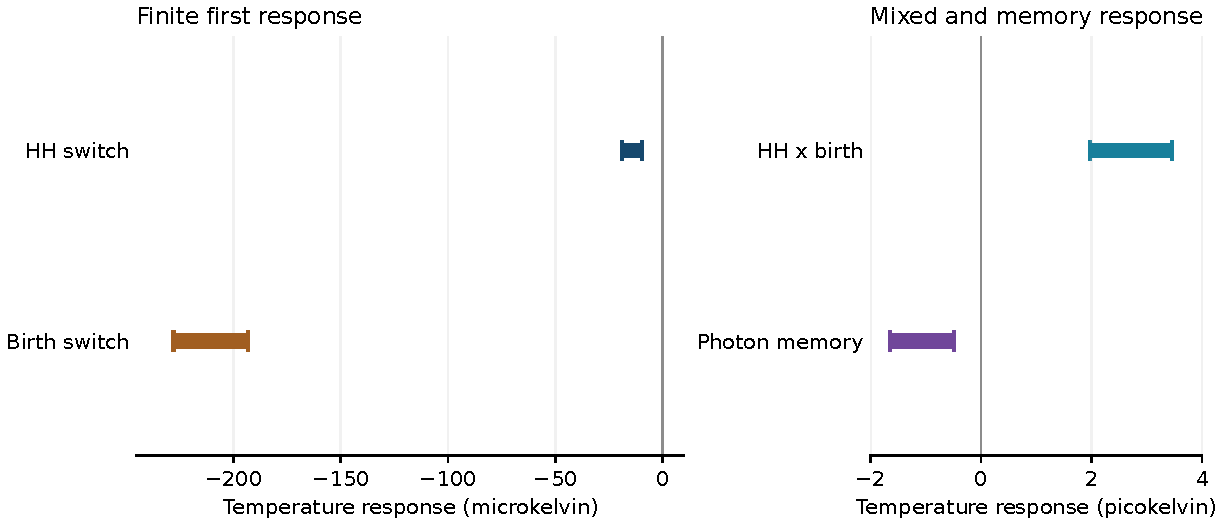
\includegraphics[width=\textwidth]{figures/temperature_response.pdf}
\caption{두-half endpoint의 유한 온도 응답. 선분 전체가 검증된 포함이며 중앙값 추정치를 뜻하지 않는다. 혼합 응답은 picokelvin, 일차 응답은 microkelvin으로 따로 표시했다.}
\end{figure}

\section{광자 기억이 만드는 추가 냉각}
HH가 첫 단계의 $x$를 늘리면 중성 H opacity가 줄어 잔존 광자가 늘어난다. 첫 단계의 구조적 $U_N^{\mathrm{in}}=0$에 대해
\begin{equation}
U_N^+=\frac{ha\Np}{D^2}U_x^+\ge0
\end{equation}
이며 양의 수송이 그 기억을 다음 incoming으로 전달한다. 원 결과에 남은 작은 signed rounding tails는 이번 계산에서 제거하지 않았다.

같은 $A^{-1}$를 적용하여 다음 세 항을 정의한다.
\begin{align}
U^{\mathrm{gas}}_2&=A^{-1}U_1,\\
U^{\mathrm{direct}}_2&=A^{-1}h q\vu,\\
U^{\mathrm{memory}}_2&=A^{-1}h\sum_j p_j\nu_jU_{N,j}^{\mathrm{in}},
\qquad U_2=U^{\mathrm{gas}}_2+U^{\mathrm{direct}}_2+U^{\mathrm{memory}}_2.
\end{align}
이는 원 $(\lambda,b)$ family의 한 미분을 전달 기여별로 분해한 것이다. 각 항을 다른 물리 모델의 독립 switch experiment로 정의하지 않는다. 기체 feedback은 모든 항에 같은 $A^{-1}$로 반영된다.
\begin{table}[H]\centering\footnotesize
\caption{같은 HH 첫 미분의 세 전달 기여. 각 항에 같은 implicit gas feedback을 적용했다.}
\label{tab:memory}
\setlength{\tabcolsep}{4pt}
\begin{tabular}{@{}lll@{}}\toprule
온도 응답 기여 & 포함 & 단위\\\midrule
전달 기체 & $[-11.41841001, -3.72939260]$ & $\mu\mathrm K$\\
두 번째 half 직접 HH & $[-7.51843474, -6.02213791]$ & $\mu\mathrm K$\\
전달 광자 기억 & $[-1.64909966, -0.49244340]$ & $\mathrm{pK}$\\
\bottomrule\end{tabular}
\end{table}


광자 기억 성분의 thermal 미분은
\begin{equation}
 U^{\mathrm{memory}}_w\in[1.7880442,5.6895403]\times10^{-18}\,\mathrm{eV/H}>0,
\end{equation}
이고 전자 미분은
\begin{equation}
 U^{\mathrm{memory}}_e\in[2.2283959,7.0951251]\times10^{-17}\,\mathrm{electrons/H}>0
\end{equation}
다. 두 효과를 같이 온도에 투영하면
\begin{equation}
 \boxed{U^{\mathrm{memory}}_T\in[-1.649099652,-0.4924434099]\,\mathrm{pK}<0.}
\end{equation}
실제 전체 33개 node 합의 부호를 직접 포함했으므로 높은 energy node의 raw tail을 exact-zero support로 해석할 필요가 없다.

직접 photo 방향에서는
\begin{equation}
T_g(p_j\nu_j)=\frac{C_Tp_j}{\Pi}\left(\epsilon_j-\frac{w}{\Pi}\right)
\end{equation}
이므로 작은 열 초과분을 가진 photon은 전자를 늘리며 입자당 열에너지를 낮출 수 있다. 최종 memory 부호는 이 직접 방향의 추측에만 의존하지 않고 위의 완전한 implicit 선형 포함으로 얻었다.\cite{theory,result,review}

\section{원 비균일 격자의 수송 분할 결함}\label{sec:remap}
\subsection{두 moment가 같아도 스펙트럼은 달라진다}
\(\Delta_j=E_j-E_{j-1}\), \(\alpha_j=(1-\rho)E_j/\Delta_j\)라 하자. $\rho E_j,\rho^2E_j\in(E_{j-1},E_j)$이고 $\rho E_{j-1}\in(E_{j-2},E_{j-1})$인 branch에서
\begin{equation}\label{eq:remap}
\boxed{[\R(\rho)^2-\R(\rho^2)]e_j
=\alpha_j\alpha_{j-1}\left[
\frac{\Delta_{j-1}}{\Delta_j}e_j
-\left(1+\frac{\Delta_{j-1}}{\Delta_j}\right)e_{j-1}+e_{j-2}\right].}
\end{equation}
원 captured nodes에서 $j=2,\ldots,32$의 branch를 확인했다. 양쪽 hat의 두 계수를 직접 곱하고, Full 계수 $(1+\rho)\alpha_j$와 빼면 식~\eqref{eq:remap}을 얻는다. 계수 합은 0이며 energy와의 내적도
\begin{equation}
\frac{\Delta_{j-1}}{\Delta_j}E_j
-\left(1+\frac{\Delta_{j-1}}{\Delta_j}\right)E_{j-1}+E_{j-2}=0
\end{equation}
으로 정확히 0이다. $j=1$에서는 두 번째 half에서 아래 guard로 넘어간 number·energy를 포함하면 같은 두 moment 항등식이 성립한다. $j=0$은 두 경로 모두 같은 guard로 이동한다.\cite{theory,geometry,result}

\subsection{실제 격자와 COMMON에서의 크기}
원 $\chi_H$ captured leaf는 $13.598434599702\,\mathrm{eV}$이고, 현재 provider가 처음 HI photo sigma를 양수로 반환하는 sampled node는 $E_{16}=13.6\,\mathrm{eV}$다. 이 둘을 같은 leaf로 취급하지 않는다. $\rho$는 약 $0.9999937500195312$여서 redshift 비율 변화 자체는 작지만, 촘촘한 node 간격에서 $\alpha_{16}\simeq0.4343923$이다.
\begin{table}[H]\centering\footnotesize
\caption{원 비균일 node에서의 선택된 column 분할 크기. 두 moment는 정확히 0이다.}
\label{tab:remap}
\setlength{\tabcolsep}{4pt}
\begin{tabular}{@{}lll@{}}\toprule
입력 node $j$ & $\alpha_j$ & column $\ell^1$\\\midrule
10 & $[0.434354825, 0.434354826]$ & $[0.754645597, 0.754645598]$\\
16 & $[0.434392324, 0.434392325]$ & $[0.754775908, 0.754775909]$\\
17 & $[0.006806228, 0.006806229]$ & $[0.006005711, 0.006005712]$\\
24 & $[0.006849978, 0.006849979]$ & $[0.000187517, 0.000187518]$\\
\bottomrule\end{tabular}
\end{table}


$j=16$의 한 광자에 대한 분할 차이는 대략
\begin{equation}
0.1886939771\,e_{14}-0.3773879542\,e_{15}+0.1886939771\,e_{16}
\end{equation}
이다. 모든 $j\ge2$ 중 최대 column $\ell^1$ 포함은
\begin{equation}
[0.7547759083005,\ 0.7547759083006]
\end{equation}
다. 이 값은 한 column의 정규화된 연산자 차이이며, 실제 total-spectrum 또는 기체 오차의 상대 비율로 읽지 않는다.

\begin{figure}[H]\centering
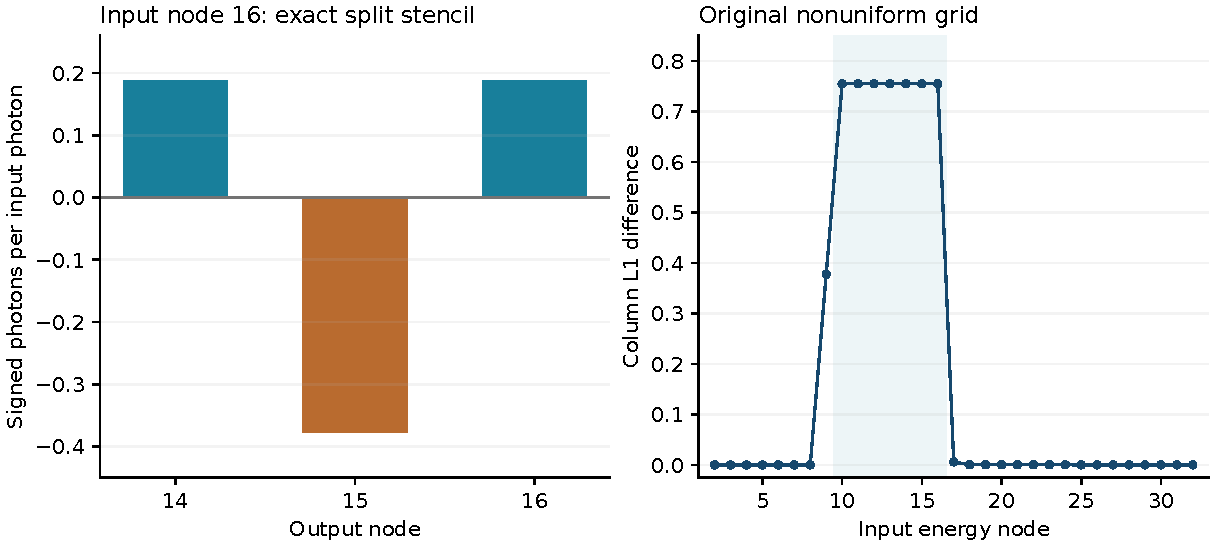
\includegraphics[width=\textwidth]{figures/remap_split.pdf}
\caption{원 격자의 수송 분할 연산자. 왼쪽은 $j=16$ column의 signed redistribution이고, 오른쪽은 $j=2,\ldots,32$ column별 $\ell^1$ 크기다. 작은 $1-\rho$만으로 원 격자의 spectral 재분배가 작다고 결론 내릴 수 없다.}
\end{figure}

원 COMMON의 실제 ray 합 스펙트럼에 \emph{차이 연산자를 먼저} 작용시키면
\begin{equation}
\delta N_{\mathrm{HI\ active}}^{\mathrm{transport}}
=\sum_{j=16}^{32}\left([\R(\rho)^2-\R(\rho^2)]N_{\mathrm{COMMON}}\right)_j
\end{equation}
가
\begin{equation}
\boxed{[-8.680771077461,-8.680422250484]\times10^{-9}\,\mathrm{photons/H}}
\end{equation}
로 포함된다. 동일 uncertain 입력을 두 번 독립 평가하여 빼는 대신 linked 차이식을 적용했으므로 COMMON 의존성의 소거가 보존된다. $j=16$ 한 column의 양의 활성-node 차이와 전체 COMMON의 음의 차이는 서로 다른 spectral 가중 결과다.

현재 수치는 absorption·birth를 제외한 수송 operator 진단이다. 두-half의 gas residual, 서로 다른 source 시각, 두 번의 birth, 중간 absorption을 모두 포함한 Full 대 two-half endpoint 결함은 다음의 결박된 비교에서 계산할 수 있다. Photon number·energy 보존만으로 그런 spectral 또는 gas 차이가 사라진다는 결론은 나오지 않는다.

\section{계산 증거, 독립 판정 및 DAG 갱신}
\subsection{실행과 포함 산술}
원 binary64 bits 및 PHYS09/11/13의 정확한 유리수 끝점을 읽고, 각 구간 연산 뒤 256 significant binary bits의 dyadic endpoints로 바깥쪽 반올림했다. 지수 범위는 제한하지 않았다. 저장된 signed tiny tails가 binary64 underflow로 소실되는 문제를 피하면서 포함을 유지한다. 이 새 산술 정밀도는 원 물리 상수나 native source 정밀도의 변경을 의미하지 않는다.

첫 scientific run의 wall time은 $0.667\,\mathrm s$, user+system CPU는 $0.639\,\mathrm s$, 최대 RSS는 $41{,}016\,\mathrm{KiB}$였다. 예산은 wall/CPU $90\,\mathrm s$, address space $768\,\mathrm{MiB}$다. 새 implicit stage 한 개가 첫 시도에 통과했고 원 성공 suite를 다시 실행하지 않았다. 초월 원자 source callback과 native root call은 실행하지 않았다. 기존 Full source inclusion을 재사용하면서 새 잔차·근·carry를 실제 계산했다.\cite{run,result}

입력 파일 45개의 SHA256과 Git blob identity를 manifest에 남겼다. NCP07 archive를 실제 복구해 원 binary layout·leaf identity를 연결했고, PHYS11 carry는 pinned Git blob과 일치했다. 한 읽기 전용 초기 schema probe의 KeyError 및 경로 정규화 사건은 별도 intake 기록에 남았다. 과학 계산의 실패나 변경으로 세지 않는다.\cite{intake}

\subsection{독립 검토의 최종 범위}
독립 검토자는 후보 프로그램을 import하거나 재실행하지 않고 별도의 380+ bit 유리수 구간 산술로 실제 source, root refinement, Neumann tail, U/V/W, T/e, carry 및 remap 포함을 확인했다. 2,713개 산술 assertion과 기하학의 528개 assertion이 통과했으며 이 반복 좌표 검사는 독립 물리 case 수에 더하지 않았다. 별도 analytic quadratic branch 및 directed-rounding oracle도 후보 측 검증 자료로 보존했다.

최종 판정은 \texttt{PROMOTE\_SCOPED}다. 원 source inclusion과 첫 단계 C2/근 계열을 상속하며, 이번에 새로 닫힌 범위는 같은 geometric isotropic subfamily의 연속 두-half 이력, 두 번째 implicit stage의 존재·유일성, global λ/b 일차·혼합·유한 관측량 응답, source-aligned aggregate carry 및 원 격자의 transport operator 진단이다. 코드와 수치 결과는 첫 성공 실행 뒤 변경하지 않았다. 이론 식 (23)의 쉼표 두 개는 수학 항을 유지한 편집 수정으로 따로 기록했다.\cite{review}


\subsection{다음 연구의 우선순위}
PHYS13까지의 기존 DAG node와 의존관계를 유지하고, 독립 provider-observable 경로에 PHYS14의 실제 carried second-half 결과를 더한다. 전체 REI critical path나 singlet 미시 원자 경로에 새로운 prerequisite를 만들지 않는다. 실제 이어진 두-half가 생겼으므로 다음 물리 질문은 \textbf{같은 COMMON 및 계수에서 Full과 two-half의 endpoint 결함을 상관관계를 보존하여 포함하는 것}이다.\cite{dag}

후속 최소 작업은 세 부분이다. 첫째, PHYS14의 두-half carry와 기존 Full의 같은 geometric subfamily를 결박한다. 둘째, 공통 입력을 보존한 defect residual 또는 Taylor difference를 구성하여 넓은 독립 root box를 단순히 빼는 손실을 줄인다. 셋째, 식~\eqref{eq:remap}의 spectral 기여, 중간 absorption, source 시각·birth chronology의 기여를 같은 endpoint 관측량으로 전달한다. 이미 확보한 group/guard와 source 미분은 재사용한다.

새 root domain 밖에서 fresh source inclusion이 필요한 지점이 생기면 해당 source 평가만 추가한다. 원 격자 비교와 관측량 결함을 먼저 판정한 뒤, 격자 변경·다단 수렴률 연구의 필요성을 결정한다. 두 시간 분할만으로 전역 수렴 차수나 EoR 오차를 확정하지 않는다. 이번에 얻은 39-state closure와 원 격자 defect 식은 그 후속 비교를 구체적으로 구성한다.

\section*{결론}
상속한 HH first\_half 결과를 실제 다음 half로 전달하여 같은 전역 제어변수의 유한 전자 증가, 온도 감소, 양의 mixed 온도 interaction을 포함했다. 전달 광자 기억은 열에너지 증가와 동시에 추가 냉각을 유발한다. 등방 source-aligned 계열에서는 39개 상태로 이 물리적 기억을 정확히 전달할 수 있다. 원 격자의 두 moment 보존과 spectral 재분배의 차이를 정량화했으므로, 다음 루프는 이미 계산한 Full 및 two-half의 상관된 endpoint 결함을 판정하는 데 집중할 수 있다.

\begin{thebibliography}{99}\fontsize{9}{10.7}\selectfont
\setlength{\itemsep}{2pt}\setlength{\parskip}{0pt}
\bibitem{result} PHYS14 actual calculation, \path{results/advance01/ADVANCE_RESULTS.json}; 요약 \path{results/advance01/SUMMARY.json}. 결과 SHA256: \path{a0faac7d55b425ae85ed8ee15e57d5f3c2687b40896b039fe858dcfdb342e28e}. 표·그림은 이 결과에서 생성했다.
\bibitem{theory} PHYS14 derived theory, \path{theory/THEORY_CANDIDATE_KO.md}, §§2--7; \path{theory/THEORY_EXACT_CHECKS.json}. 기존 PHYS11 chain rule 및 PHYS13 readout은 재사용으로 귀속했다.
\bibitem{phys11} PHYS11, \path{inputs/phys11/CARRY_RESULTS.json}, first\_half outgoing\_joint; \path{inputs/phys11/JOINT_CARRY_DERIVATION_KO.md}; \path{inputs/phys11/SOURCE_TO_CARRY_MAP_KO.md}. Pinned carry SHA256: \path{5e3dc0b589c5e86672664ea851e7986708e10ed73f6a3db8332b9c8084a897ca}.
\bibitem{phys13} PHYS13, \path{inputs/phys13/THERMO_RESULTS.json}, first\_half root\_image; \path{inputs/phys09/PROJECTED_RESULTS.json}, first\_half $U,V,W$. PHYS13 직전 PR: \url{https://github.com/cosmosapjw-quantum/WU088_HH/pull/48}.
\bibitem{ncp07} NCP07 pinned archive 및 \path{inputs/ncp07/results/full/}, \path{inputs/ncp07/results/first_half/}. Energy/sigma/heat, source native leaves, C2 domain, PREBE bits, ray/guard binary payload와 geometry trace.
\bibitem{source} 원 source, \path{inputs/ncp07/candidate/src/phys04_mixed.rs}, \path{phys04_transport.rs}, \path{paired_runtime.rs}; \path{inputs/ncp07/src/sourcebox.rs}. 실제 읽은 함수·파일 범위는 \path{theory/SOURCE_READ_SCOPE.json}에 기록했다.
\bibitem{geometry} 독립 geometry 검토, \path{review/GEOMETRY_REVIEW.json}, \path{review/geometry_review.py}. 실제 geometric common ratio 및 정상화 source weight의 원 128 ray 구간 포함, 원 branch 및 remap 항등식.
\bibitem{run} 실행 전 계약·검증 행렬, \path{SCIENTIFIC_CONTRACT.md}, \path{VALIDATION_MATRIX.md}; 실제 실행 \path{evidence/advance01/PRE_RUN.json}, \path{RUN_RECORD.json}, stdout/stderr 및 source identity.
\bibitem{review} 독립 최종 검토, \path{review/DECISION.json}, \path{review/REVIEW_KO.md}; 검토자의 실제 수치 재구성과 source·산술 결박은 부속 검토 결과에 기록했다.
\bibitem{intake} 원자료 복구·identity, \path{inputs/INPUT_MANIFEST.json}, \path{inputs/intake/INTAKE_PROVENANCE.json}, \path{SOURCE_IDENTITY.json}, \path{BINARY_LAYOUT_VERIFICATION.json}, \path{PHYS11_CARRY_IDENTITY.json}.
\bibitem{dag} PHYS14 연구 DAG, \path{NEXT_DAG.json}; 직전 원문 \path{inputs/phys13/NEXT_DAG.json}. 기존 node는 보존하고 provider 결과와 구체적인 다음 결함 계산만 추가한다.
\end{thebibliography}
\end{document}
